\chapter{Arbeitsablauf und Problematiken}
\label{cha:Workloop}

Der Arbeitsablauf des Roboters kann in unterschiedliche Phasen unterteilt werden. Diese Phasen sind als in Abbildung als Petrinetz beschrieben.

\begin{figure}[h]
\centering
\caption{Petrinetz des Arbeitsablaufs}
\label{fig:Petrinetz}
\end{figure}

Die Arbeitsweise sowie auftretende Probleme sind in den folgenden Abschnitten beschrieben.

\section{Objektsuche}

%\section{Objektverfolgung}

Sobald mehrere Objekte durch die in Kapitel \ref{sec:Objekterkennung} dargestellten Algorithmen erkannt wurden, muss eines als geeignetes Fokusziel gewählt werden. Diese Wahl erfolgt auf Basis der Form des Objektes, wobei versucht wird ein möglichst kompaktes Objekt auszuwählen, dass sich in der Bildmitte befindet

TODO Hier kann noch mehr rein


Damit der Roboter nicht ständig sein Ziel wechselt, muss er das Fokusobjekt in nachfolgenden Aufnahme wiedererkennen. Ein zufälliges Umspringen auf zufällige andere erkannte Objekte wäre für den Prozess sehr hinderlich. In den folgenden Abschnitten sind Kriterien und Probleme beschrieben, an Hand derer ein erkanntes Objekt in folgenden Aufnahmen erkannt werden kann. Das Fokusobjekt wird von der Applikation durch ein grünes Rechteck, andere gefundene Objekte durch ein rotes markiert. Dieses Vorgehen ist in Abbildung \ref{fig:Markierung} dargestellt.

\begin{figure}[h]
\centering
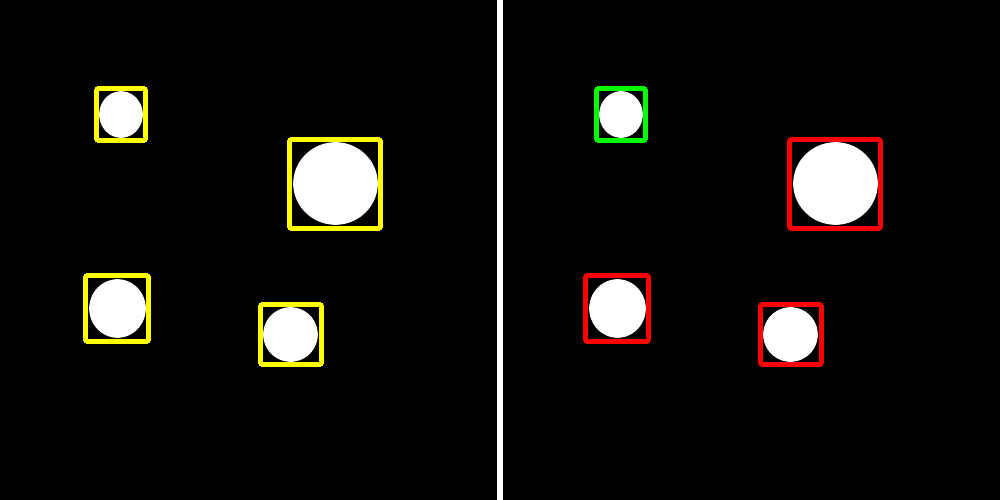
\includegraphics[width=0.8\textwidth]{Bilder/Workloop/Markierung}
\caption{Auffindung eines Fokusobjekts}
\label{fig:Markierung}
\end{figure}

\subsection{Ähnlichkeitskriterien}
\label{subsec:Similarity}
Um den Fokus auf ein Objekt zu behalten lassen sich verschiedene Ähnlichkeitskriterien formulieren durch die das erkannte Objekt in der Menge der im nachfolgenden Bild erkannten Objekte wieder gefunden werden kann.



\subsubsection{Lokale Nähe}
Das trivialste Kriterium stellt die lokale Nähe da. Geht man von einem Stillstand der Kamera und der aufgenommenen Szene aus, so befinden sich sämtliche Objekte in nachfolgenden Aufnahmen an der selben Stelle. Fokussierte Objekte können daher rein aus ihrer Position wiedergefunden werden. Ist das System in Bewegung, so kann nicht mehr von einer exakten Übereinstimmung der Koordinaten ausgegangen werden. Stattdessen wird eine gewisse Toleranz gegeben. Als Maß kann hierbei angenommen werden, dass sich die Position des Zentrums eines Objektes in fortlaufenden Aufnahmen um nicht mehr als beispielsweise 10\% der Aufnahmegröße geändert hat. Abbildung \ref{fig:LokaleNaehe} zeigt das beschriebene Verhalten anschaulich am Beispiel einer nachfolgenden Aufnahme aus Abbildung \ref{fig:Markierung}. 

\begin{figure}[h]
\centering
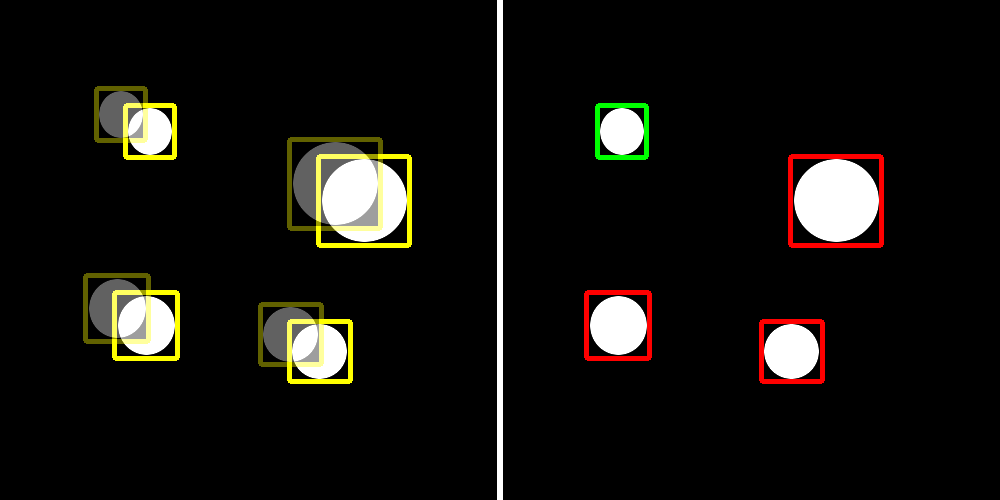
\includegraphics[width=0.8\textwidth]{Bilder/Workloop/MovingMarker}
\caption{Objektverfolgung durch Kriterium der lokalen Nähe}
\label{fig:LokaleNaehe}
\end{figure}

\subsubsection{Größenkriterium}
Das Größenkriterium ähnelt zunächst dem Kriterium der lokalen Nähe, bezieht sich jedoch nicht auf den Mittelpunkt des Objekts, sondern auf die vom Objekt in der Aufnahme eingenommenen Fläche. Diese bleibt bei einer beliebigen Translation des Objektes in der Aufnahme konstant und eignet sich daher als Ähnlichkeitsmaß. Bewegt sich das Objekt jedoch auf die Kamera zu, oder von ihr weg, so verändert sich die eingenommene Fläche. Auch hier muss eine Toleranz gewählt werden. Dise kann entweder konstant gegeben sein (beispielsweise 10\%) oder abhängig von der aktuellen Geschwindigkeit des Roboters gewählt werden. Abbildung \ref{fig:GroessenKriterium} zeigt exemplarisch die Verfolgung eines Objektes dessen Größe sich im Verlauf der Aufnahmeserie verändert.

\begin{figure}[h]
\centering
\caption{Objektverfolgung durch Größenkriterium}
\label{fig:GroessenKriterium}
\end{figure}

\subsubsection{Farbliche Ähnlichkeit}
Ein drittes Ähnlichkeitsmaß stellt die farbliche Ähnlichkeit dar. Diese ist Abhängig vom Farbraum in dem die Aufnahme getätigt oder konvertiert wurde. Wie in Abschnitt \ref{sec:Objekterkennung} beschrieben, wird die Aufnahme bei der Objekterkennung in das HSV-Format konvertiert. Daher kann das Ähnlichkeitsmaß sich auf den Farbkanal, den Sättigungskanal oder den Intensitätskanal beziehen. Durch außschließen des Intensitätskanals kann eine weitgehend helligkeitsunabhängige Bestimmung erreicht werden. Daher ist das Filtern nach Objekten ähnlicher Farbe und Sättigung durchaus sinnvoll. Auch hier lässt sich eine Toleranz formulieren, wie etwa 10\% Abweichung von der durchschnittlichen Farbe des zuvor ermittelten Objektes. Abbildung \ref{fig:FarbKriterium} zeigt die farbliche Ähnlichkeit zweier Objekte und die dadurch resultierende Wiederfindung des Objektes in der Folgeaufnahme.

\begin{figure}[h]
\centering
\caption{Objektverfolgung durch farbliche Ähnlichkeit}
\label{fig:FarbKriterium}
\end{figure}

\subsection{Kurzzeitiger Verlust des Verfolgungsziels}

Tendenziell muss bei der Objektverfolgung immer von einem Verlust des verfolgten Objektes ausgegangen werden. Dies kann permanent sein, wie beispielsweise bei apprupter starker Veränderung der Lichtbedingungen, oder lediglich temporär durch Fehler bei der Bildaufnahme geschehen. In diesem Abschnitt wird auf letzteres eingegangen, da das Verhalten bei längerfristigem Verlust wird in Abschnitt \ref{sec:MainLoop} beschrieben wird.

Es hat sich gezeigt, dass kleine Fehler oder Ungenauigkeiten bei der Bildaufnahme bereits dazu führen können, dass ein Objekt nicht in der darauf folgenden Aufnahme wiedergefunden werden kann. Ist dies nur von kurzer Dauer, muss dies gesondert behandelt werden um zu vermeiden, dass der Roboter einen plötzlichen Wechsel des Verfolgungsziels durchführt. Ähnlich der in Abschnitt \ref{subsec:Similarity} beschriebenen Ähnlichkeitskriterien muss auch hier eine Toleranz für eine maximale Anzahl Aufnahmen gelegt werden, in denen das verfolgte Ziel nicht gefunden werden muss ohne, dass das Objekt als "verloren" angesehen wird. Die Wahl einer zu hohen Toleranz hat die Folge, dass der Roboter lange Zeit in einem undefinierten Zustand ein Objekt verfolgt, welches er nicht sieht. Ist die Schwelle zu niedrig gewählt, so kann dies ein häufiges Springen zwischen verschiedenen Objekten zur Folge haben, was sich sehr negativ auf die Laufzeit auswirken könnte. Empirisch hat sich gezeigt, dass eine solche Schwelle bereits bei etwa drei Aufnahmen ohne das verfolgte Objekt liegen kann. Wird ein Objekt verloren, so begibt sich der Roboter zurück in den Zustand der Objektsuche.


\subsection{Verzerrte Aufnahmen durch Bewegung des Roboters}

Durch Bewegung des Roboters während der Bildaufnahme, kann es zu verzerrten Bildern kommen. Dies kann unterschiedliche Folgen haben. Abbildung \ref{fig:Verzerrung} zeigt eine solche verzerrte Aufnahme. 

\begin{figure}[h]
\centering
\caption{Verzerrte Aufnahme durch Bewegung des Roboters}
\label{fig:Verzerrung}
\end{figure}

Durch die Verzerrung können unterschiedliche Phänomene auftreten. Die Verfolgung von Objekten, die in Abschnitt \ref{subsec:Similarity} beschrieben wurde kann versagen. In diesem Fall muss die Aufnahme ignoriert und verworfen werden. Es können jedoch auch Objekte fälschlicherweise erkannt und kategorisiert. Durch die Verzerrung wird die Form und Position der Objekte verfälscht. Eine solche verfälschte Aufnahme kann einen plötzlichen Wechsel des fokussierten Objektes zur Folge haben.

\section{Anfahren von Objekten}
\label{sec:Ansteuerung}

Sobald ein Objekt gefunden wurde, kann der Roboter beginnen dies anzufahren. Hierfür versucht er zunächst das Objekt horizontal zu zentrieren. Dafür dreht sich der Roboter auf der Stelle, bis das Objekt ganz zu sehen ist und das möglichst zentral in der Aufnahme liegt. Abbildung \ref{fig:Zentrierung} zeigt, wie ein Objekt durch die Drehung des Roboters zentriert werden konnte.

\begin{figure}[h]
\centering
\caption{Zentrierung eines Objekts}
\label{fig:Zentrierung}
\end{figure}

Ist das Objekt zentral gelegen, so muss der Roboter lediglich geradeaus fahren, bis er es erreicht. Da eine perfekte Zentrierung jedoch nicht garantiert werden kann, ist es möglich, dass der Roboter abdriftet. Um dem vorzubeugen muss ständig die Position des Objekts in der Aufnahme überprüft und gegebenenfalls zentriert werden.

Weiterhin wichtig, ist es jedoch zu wissen, wann in den Zustand des Objekt Aufhebens übergegangen werden kann. Hierfür darf der Roboter nur eine geringe Entfernung zum Objekt aufweisen. Die folgenden Abschnitte gehen auf verschiedene Methoden der Entfernungsmessung ein.

\subsection{Entfernungsschätzung}
Die Entfernungsschätzung ist für mehrere Teile der Roboterroutine wichtig. Zunächst muss der Roboter, der ein Objekt per Kamera erkannt hat anfahren und aufheben. Hierfür muss er wissen ob der aufzuhebende Gegenstand in Reichweite des Greifarms ist. Weiterhin benötigt der Roboter die Entfernungsschätzung bei der Navigation. Er muss Hindernisse, wie beispielsweise Wände eines Raumes, erkennen bevor er kollidiert und unter Umständen seine Fracht verliert.

\subsubsection{Stereokamerabasiert}
\label{subsec:StereoKameraDist}

Ein häufiger Ansatz für die Entfernungsschätzung stellt die Stereokamerabasierte Methode dar. Hierbei nimmt der Roboter seien Umgebung nicht mit nur einer Kamera, sondern mit mehreren, mindestens zwei, wahr. Durch einen bekannten Versatz zwischen den Aufnahmequellen der Bilder, lässt sich mittels Registrierung auch ein Versatz in den erzeugten Bildern ermitteln. Wie die beiden menschlichen Augen, erlaubt dies das Wahrnehmen der Umgebung in dritter Dimension. Abbildung \ref{fig:StereokameraEntfernung} zeigt schematisch eine solche Entfernungsschätzung \cite{bathge20123d}.

\begin{figure}[h]
\centering
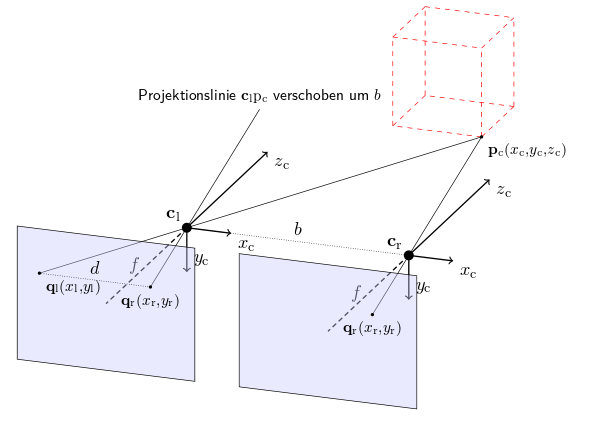
\includegraphics[width=0.8\textwidth]{Bilder/Workloop/Stereokamera}
\caption{Stereokamerabasierte Entfernungsschätzung}
\label{fig:StereokameraEntfernung}
\end{figure}

Der Stereokamerabasierte Ansatz ist von der Ausführung sehr elegant, da er sich an der Natur und dem menschlichen räumlichen Sehen orientiert. 

Problematisch ist jedoch, dass zusätzliche Hardware benötigt wird. Eine weitere Kamera als bildgebendes Mittel birgt einen neuen Grad der Komplexität, da diese mit dem vorhandenen Smartphone synchronisiert werden muss. Zusätzlich müssen zeitintensive Berechnungen durchgeführt werden, wodurch die Echtzeitfähigkeit des Systems beeinträchtigt werden könnte.

\subsubsection{Monokamerabasiert}

Der Monokamerabasierte Ansatz stützt sich bei der Entfernungsberechnung auf alle vorhandenen Informationen. Hierbei wird mittels der bekannten Position und Inklination der Kamera, sowie ihres Streuwinkels ein virtuelles Blickfeld erstellt. Dieses Blickfeld breitet sich von der Kamera aus pyramidenförmig aus und trifft den als planar angenommenen Boden. Abbildung \ref{fig:MonokameraEntfernung} zeigt den Aufbau eines solchen Systems. 

\begin{figure}[h]
\centering
\caption{Monokamerabasierte Entfernungsschätzung}
\label{fig:MonokameraEntfernung}
\end{figure}

Anhand der Position des detektierten Objektes im Kamerabild lässt sich daraufhin eine ungefähre Entfernungsschätzung liefern. Problematisch ist hierbei die Ungenauigkeit des Systems. Sowohl Fehler bei der Aufnahme, als auch Probleme durch eine maximale Größenbeschränkung des detektierten Objektes können in der Praxis zu Fehleinschätzungen und damit fehlerhafter Benutzung des Greifarms führen. 

In den von uns durchgeführten Tests, konnte lediglich eine Genauigkeit von $\pm 5cm$ erreicht werden. Dies ist für die gegebene Anwendung unzureichend.

\subsubsection{Ultraschallbasiert}
\label{subsec:Ultraschall}

Die ultraschallbasierte Entfernungsschätzung kann auch über große Distanzen von bis zu zwei Metern zentimetergenaue Entfernungen messen. Die Messung wird durch einen Echo-Mechanismus mit, für den Menschen unhörbaren, Schallwellen im Ultraschallbereich durchgeführt \cite{hertzberg2012mobile}. Zunächst wird jedoch, ähnlich dem in \ref{subsec:StereoKameraDist} beschriebenen Verfahren, zusätzliche Hardware in Form eines Ultraschallsensors benötigt. Ein solcher kann jedoch direkt von LEGO\texttrademark\ erworben und problemlos am Roboter angebracht werden. 

Das ultraschallbasierte Verfahren kann durch eine kleine Änderung des Roboters realisiert werden und liefert sehr genaue Ergebnisse. Die Koppelung mit dem Smartphone ist bereits gegeben und genügt Echtzeitanforderungen.

\section{Aufnehmen von Objekten}
\label{sec:Aufnehmen}

Das Aufnehmen von Objekten kann erfolgen sobald der Roboter, wie in Abschnitt \ref{sec:Ansteuerung} beschrieben, nah genug an das Objekt herangefahren ist. Zum Aufnehmen wird der Greifarm durch das Betreiben des dritten Motors geschlossen. Näheres hierzu findet sich im Kapitel \ref{sec:Greifarm}. 

Mit Hilfe des in Abschnitt \ref{subsec:Ultraschall} beschriebenen Ultraschallsensors kann ebenfalls überprüft werden ob das Objekt während des Tragens verloren geht. In diesem Fall kehrt der Roboter zurück in den Zustand der Objektsuche.

\section{Kategorisierung von Objekten}

Objekte werden nach zwei Kriterien kategorisiert. Diese Kriterien sind in den folgenden Abschnitten näher beschrieben.

\subsection{Kategorisierung nach Farbe}
Die Farbe des Objekts stellt ein Kriterium dar. Diese wird über die gesamte Objektverfolgung ermittelt. So kann akkurat eine beleuchtungsunabhängige Kategorisierung in menschlich wahrnehmbare Farben stattfinden. Tabelle \ref{tab:Farbtabelle} beschreibt die Auswertung der im HSV Farbraum ermittelten Farbwerte.

\begin{table}
	\centering
	\begin{tabular}{lr}
		\toprule
		Farbe & HSV-Kriterium\\
		\midrule
		Rot & $H < 15\vee H \geq 160$ \\
		Orange & $15 \leq H < 20$ \\
		Gelb & $20 \leq H < 35$ \\
		Grün & $35 \leq H < 60$ \\
		Blau & $60 \leq H < 140$ \\
		Violett & $140 \leq H < 160$ \\
												
		\bottomrule
	\end{tabular}
	\caption{Umrechnung von HSV-Werten in konkrete Farben.}
	\label{tab:Farbtabelle}
\end{table}

In jeder Aufnahme wird die konkrete Farbe des Objekts bestimmt. Anschließend kann bei der Kategorisierung die am häufigsten bestimmte Farbe gewählt werden um Fehler durch Beleuchtung oder andere äußere Einflüsse zu korrigieren.

\subsection{Kategorisierung nach Form}
TODO

\section{Suche des Zielbereichs}
\subsection{Orientierung im Raum}
\label{subsec:Orientierung}
\subsubsection{Kameragestützt}
\subsubsection{Streckenbasiert}
Über gefahrene Strecke

\section{Ansteuerung des Zielbereichs}
\section{Ablegen von Objekten}
Das Ablegen von Objekten erfolgt analog zum in Abschnitt \ref{sec:Aufnehmen} beschriebenen Aufnehmen von Objekten. Sobald die Zielzone erreicht wird, kann das getragene Objekt abgelegt werden. Dies erfolgt über die Ansteuerung des dritten Motors, der den Greifarm steuert. 

Sobald das Objekt an der Zielzone abgelegt wurde, kann der Roboter zurück an seine Ausgangsposition fahren. 

\section{Rückkehr zur Ausgangsposition}

Mit Hilfe der in Kapitel \ref{subsec:Orientierung} beschrieben Verfahren kann sich der Roboter im Raum orientieren und den Startpunkt ausfindig machen und ansteuern. Abbildung \ref{fig:Startpoint} zeigt einen Screenshot der Applikation sobald der Roboter in die Ausgangsposition zurückzukehren versucht. 

Sobald der Roboter die Ausgangsposition erreicht hat, ist ein Zyklus seines Arbeitsablaufs abgeschlossen. Durch Wiederholen der in diesem Kapitel beschriebenen Schritte kann ein weiteres Objekt detektiert, kategorisiert und in eine Zielzone transportiert werden. 

\begin{figure}[h]
\centering
\caption{Screenshot der Applikation bei Rückkehr zur Ausgangsposition}
\label{fig:Startpoint}
\end{figure}